En este capítulo, veremos el diseño del sistema así como la interacción que tienen los distintos componentes entre sí.

\newpage

\section{Arquitectura lógica}
La arquitectura lógica de nuestro sistema esta íntimamente ligada a la arquitectura propia de cualquier software que usa los servicios de una cloud pública como Azure, es decir, basado en servicios y distribuido.

Además, debido a que nuestro proyecto tiene 2 grandes componentes o subsistemas, explicaremos la arquitectura de cada uno de ellos. Por un lado, explicaremos y detallaremos la arquitectura del Sistema de Gestión y, por el otro, la del Sistema de IoT.

\subsection{Sistema de Gestión}
Para el Sistema de Gestión, se ha desarrollado una arquitectura con sistemas distruidos, donde el código tanto del frontend, como backend o la base de datos, no tiene porqué esta alojados en el mismo sitio. De hecho, no lo están.

Como todo buen sistema distribuido, los distintos componentes se tienen que comunicar entre sí. Esto se hace mediante REST API, donde el backend recibe datos y este devuelve una respuesta confirmando su correcto o incorrecto procesamiento.

A continuación, en la Figura 5.1 se muestra de forma breve y concisa la arquitectura entre el Frontend y el Backend.

\begin{figure}[H]
    \centering
    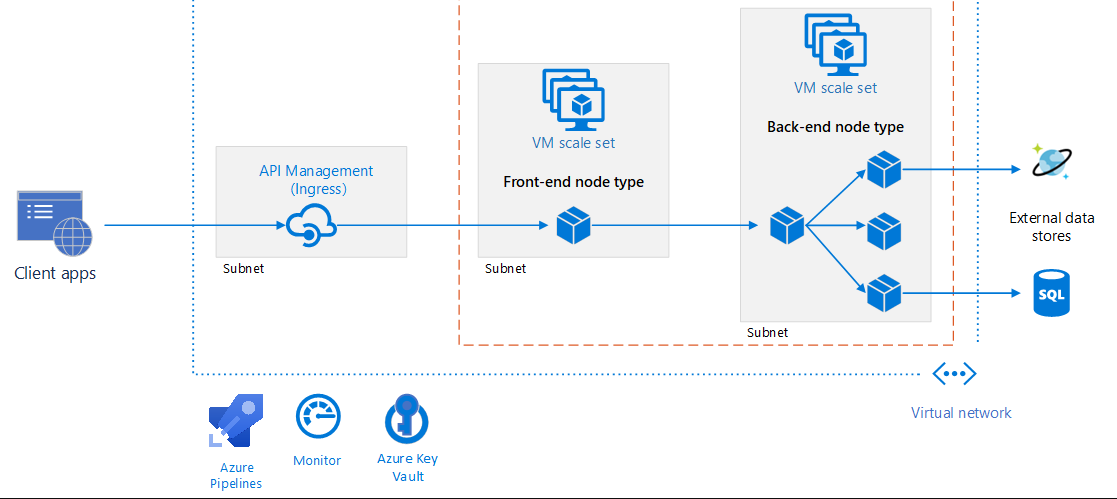
\includegraphics[width=1\linewidth]{images/design/front-back.png}
    \caption{FrontEnd + Backend \cite{frontbackazure}}
\end{figure}

Pero, no solo de esto se nutre la arquitectura del sistema, ya que, también tendriamos que incluir el proceso de Integración Continua / Distribución Continua (Continuous Integration and Continuous Delivery, CI/CD \cite{cicd}) que se encarga de los despliegues automatizados para evitar esa pesada, repetitiva y tortuosa carga.

El CI/CD que hemos utilizado para hacer los despliegues automatizados no es más que el por defecto que tiene la plataforma GitHub. Hemos utilizado este y no Azure Pipeline debido a que lo ideal es que el mismo sistema de repositorio sea el encargado de construir la aplicación y desplegarla en la cloud, y que no sea Azure el encargado de dicha tarea. Esto es debido a que, si el dia de mañana decidimos cambiar, solo tendriamos que cambiar parte de la arquitectura o servicios que se usan, pero no el CI/CD.

A continuación, en la Figura 5.2 se muestra de forma breve y sencilla todo el proceso.

\begin{figure}[H]
    \centering
    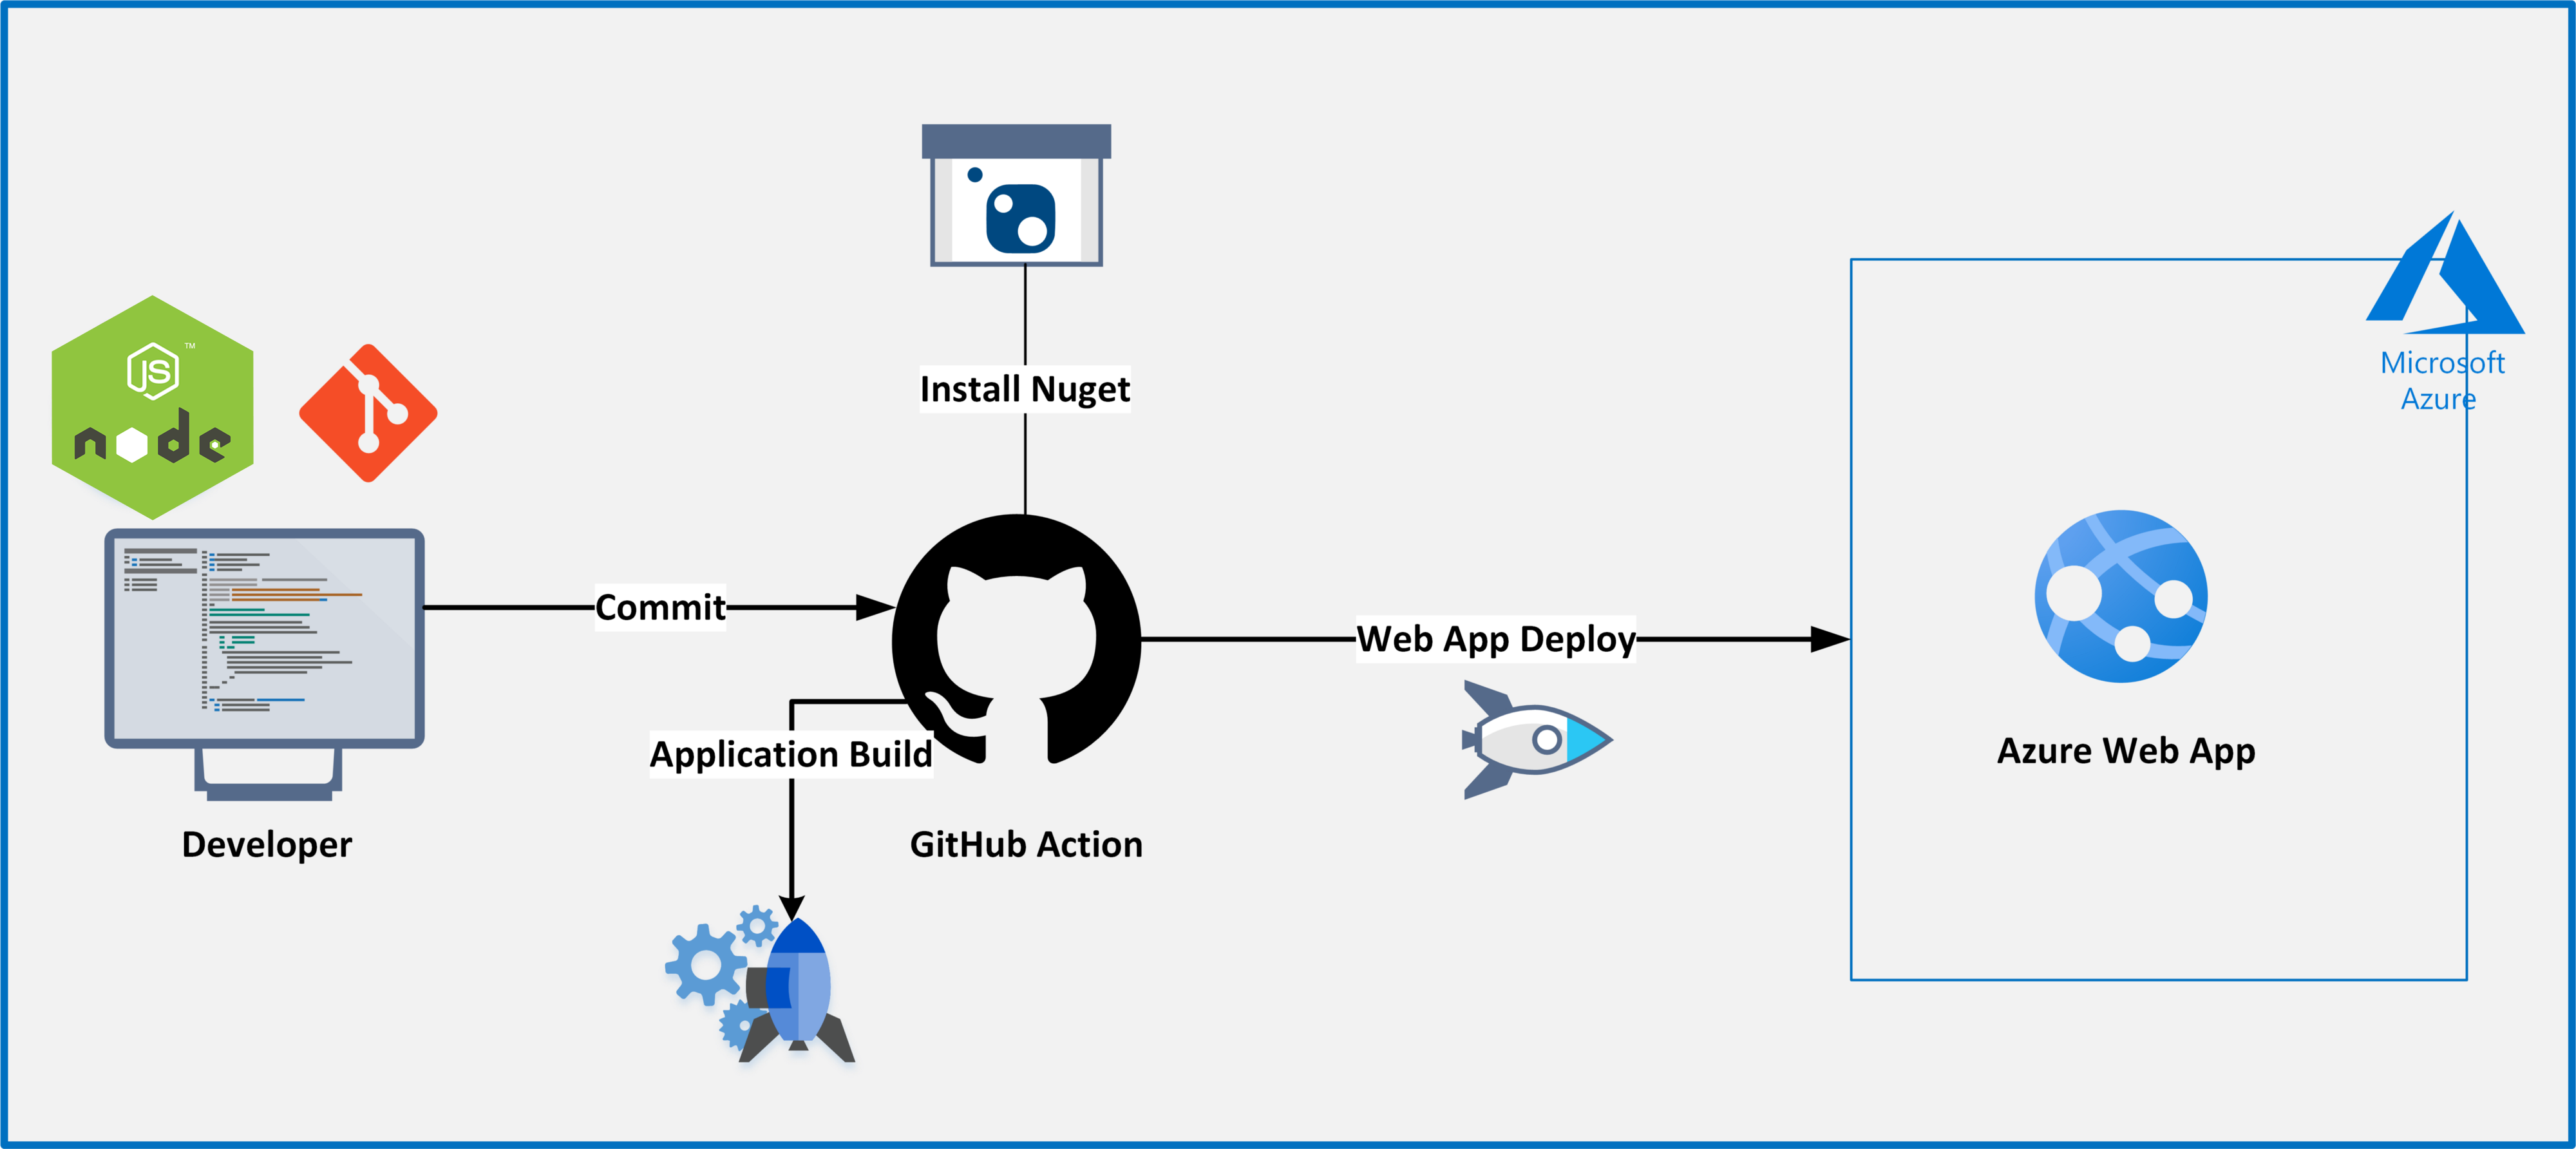
\includegraphics[width=1\linewidth]{images/design/github azure.png}
    \caption{GitHub Workflow Action + Azure \cite{github-azure}}
\end{figure}

\subsection{Sistema de IoT}
Por otra parte, el Sistema de IoT tiene su propia arquitectura, ya que, aunque comparte plataforma, Azure Cloud, el despliegue, el funcionamiento y el mismo concepto persé cambian drásticamente al de un sistema distribuido puro del tipo backend más frontend.

Este sistema tiene una arquitectura típica de todos los sistemas de IoT, es decir, dispositivo creador de eventos simples, un procesador de patrones de eventos simples y que si el patrón coincide, dispara el evento complejo y por último, un dispositivo que este atento a los eventos complejos y ejecute la acción por defecto que tengan asignada.

A continuación, exponemos en la Figura 5.3 como y que componentes tiene este sistema de IoT con Azure Cloud.

\begin{figure}[H]
    \centering
    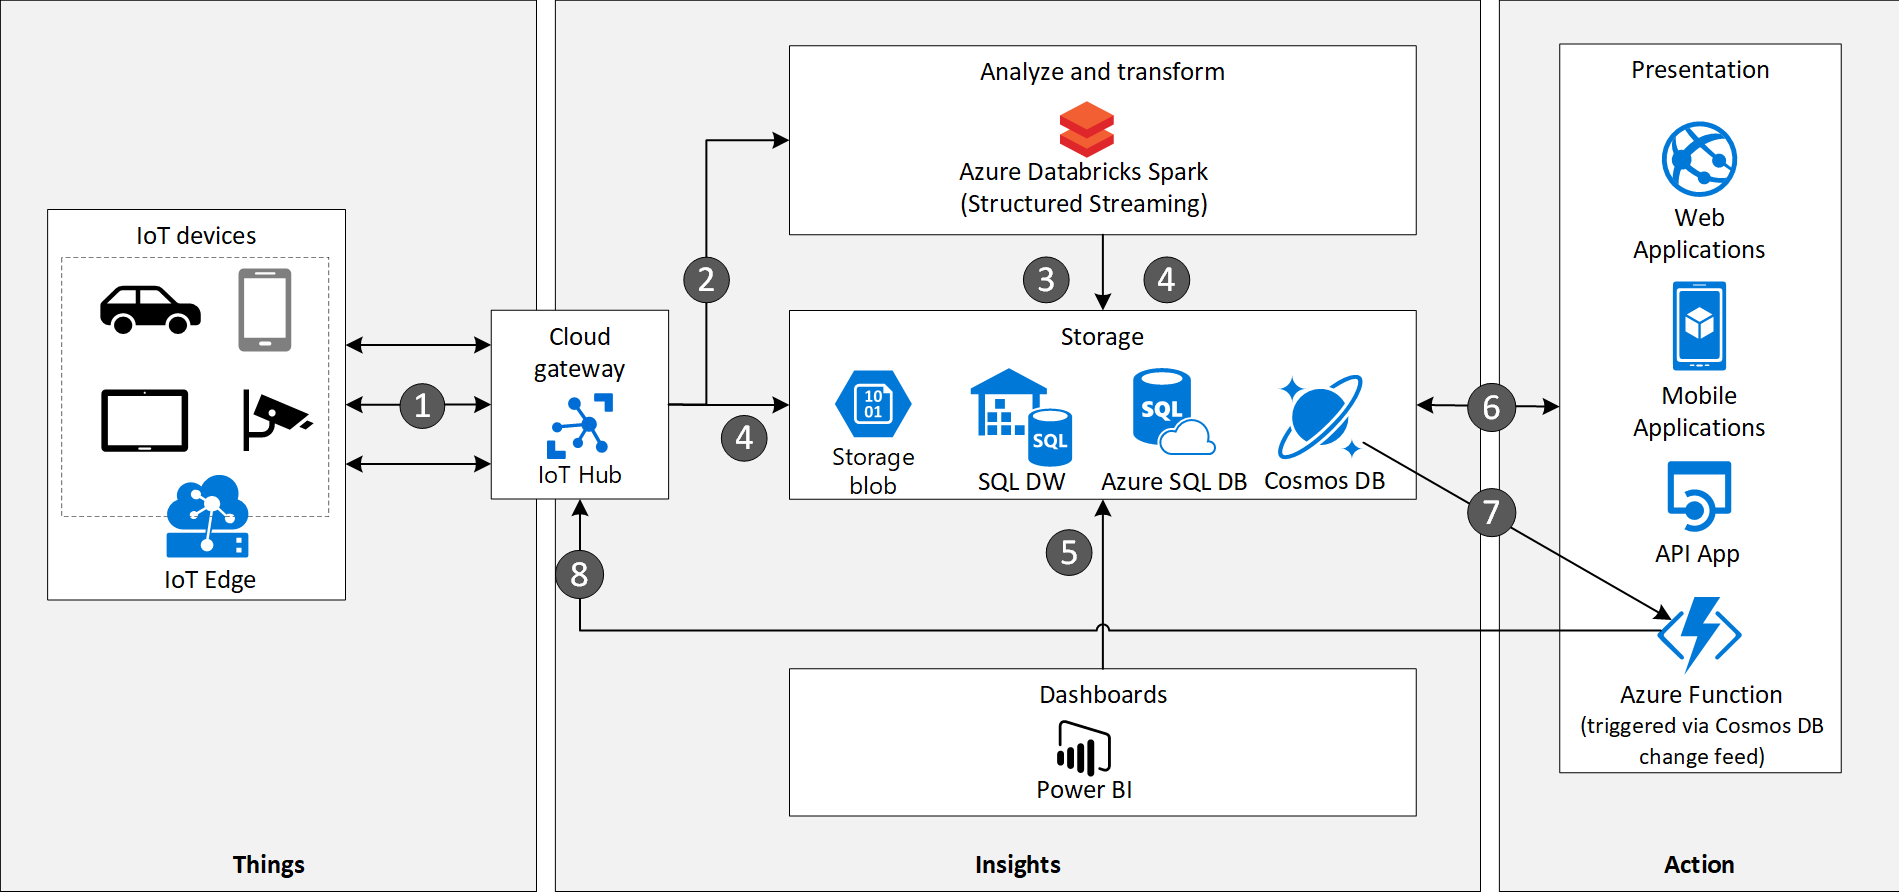
\includegraphics[width=1\linewidth]{images/design/iot-using-cosmos-db.png}
    \caption{IoT Azure \cite{iot-azure}}
\end{figure}

\section{Modelo Relacional}
En este apartado, exponemos el modelo relacional de la base de datos, es decir, que tablas posee y la relación entre las mismas. Además, mostramos las tablas y las relaciones que tienen entre sí, en las Figuras 5.4, 5.5, 5.6 y 5.7.

\begin{figure}[H]
    \centering
    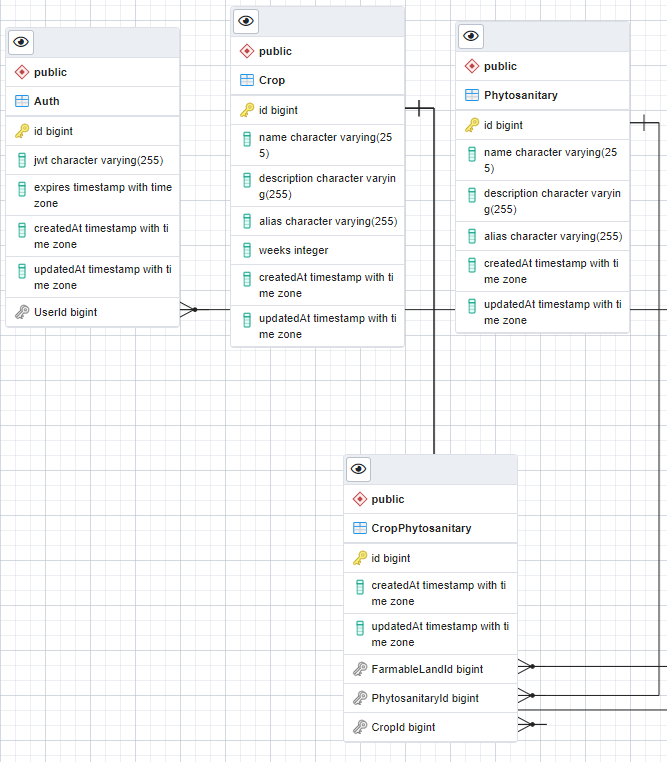
\includegraphics[width=1\linewidth]{images/design/erd1.png}
    \caption{Tablas Auth, Crop, Phytosanitary y CropPhytosanitary}
\end{figure}

\begin{figure}[H]
    \centering
    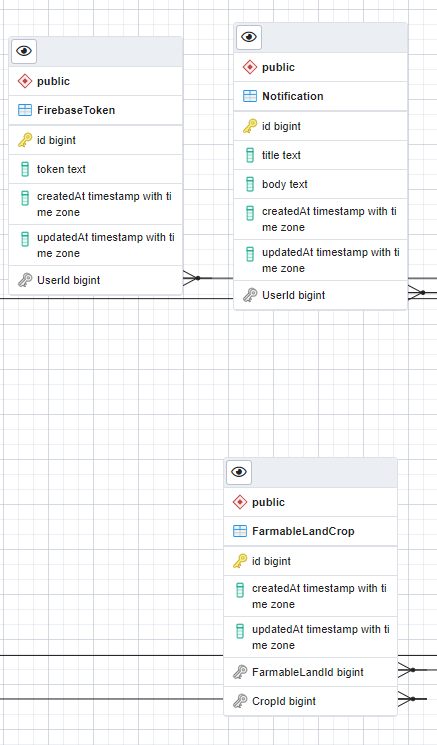
\includegraphics[width=1\linewidth]{images/design/erd2.png}
    \caption{Tablas FrebaseToken, Notification y FarmableLandCrop}
\end{figure}

\begin{figure}[H]
    \centering
    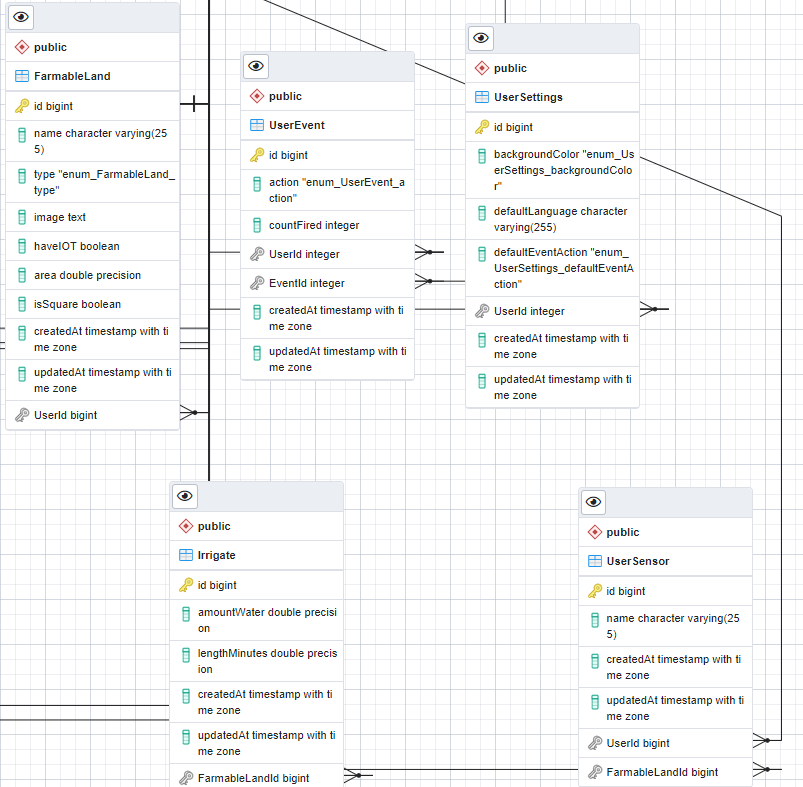
\includegraphics[width=1\linewidth]{images/design/erd3.png}
    \caption{Tablas FarmableLand, UserEvent, UserSettings, Irrigate y UserSensor}
\end{figure}

\begin{figure}[H]
    \centering
    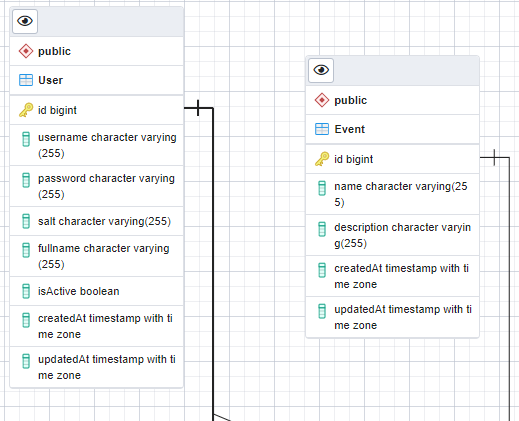
\includegraphics[width=1\linewidth]{images/design/erd4.png}
    \caption{Tablas User y Event}
\end{figure}

Además, para aclarar la composición de las tablas, listamos a continuación las mismas con sus columnas y con una breve descripción.

\begin{itemize}
    \item Auth: tabla dedicada a almacenar la información de autenticación del usuario.
    \item Crop: tabla dedicada a almacenar la información de los cultivos.
    \item Phytosanitary: tabla dedicada a almacenar la información de los fitosanitarios.
    \item CropPhytosanitary: tabla dedicada a relacionar los cultivos con los fitosanitarios.
    \item FirebaseToken: tabla dedicada a almacenar el token de dispositivo generado por firebase.
    \item Notification: tabla dedicada a almacenar las notificaciones del usuario.
    \item FarmableLandCrop: tabla dedicada a relacionar los terrenos con los cultivos.
    \item FarmableLand: tabla dedicada a almacenar los terrenos.
    \item UserEvent: tabla dedicada a relacionar los eventos complejos con un usuario.
    \item UserSettings: tabla dedicada a almacenar los ajustes del sistema del usuario.
    \item Irrigate: tabla dedicada a almacenar los riegos de los terrenos.
    \item UserSensor: tabla dedicada a relacionar sensores con usuarios.
    \item User: tabla dedicada a almacenar los usuarios del sistema.
    \item Event: tabla dedicada a almacenar los eventos complejos disponibles.
\end{itemize}

\section{Diseño de la interfaz}
Para el diseño de la interfaz, se ha usado una guía de diseño minimalista, donde predominan los espacios abiertos y con poca carga visual. Es decir, interfaz sencilla y que permita al usuario saber de un vistazo donde esta todo.

Por otra parte, como nuestro público objetivo son personas del mundo rural, se ha simplificado aún más ciertas tareas como las búsquedas, donde no se han puesto filtros ni elementos añadidos que puedan abrumar al usuario.

Además, la paleta de colores ha sido importante, ya que, uniamos las acciones peligrosas y sin vuelta atrás con el rojo, mientras que a las acciones informativas o de actualizan con capacidad de retorno, con colores más amenos como azul o verde. Todo ello, siempre en tonos claros, ya que, como se dijo anteriormente, la predominancia del color es el blanco y con colores claros no hay mucho contraste que pueda impactar de forma negativa al usuario.

Las imágenes, aunque siempre coloridas, se les ha impuesto en todos los casos un tamaño máximo para que no descuadre todos los componentes de su entorno, fácilitando así al usuario el seguir encontrado todo en su sitio y sin tener que volver a investigar donde esta todo de nuevo.

También, un elemento importante es el texto. Como siempre, hemos intentado que sean textos minimalistas, que con muy poco texto describa la situación o componente. De hecho, la parte de la aplicación que tiene más texto son las notificaciones que se envían al usuario cuando se dispara algún evento complejo.

Por último, para los componentes meramente visuales, se han usado los componentes del SDK Ionic \cite{ui-ionic}.